\documentclass{article}

\usepackage{fancyhdr}
\usepackage{extramarks}
\usepackage{amsmath}
\usepackage{amssymb}
\usepackage{amsthm}
\usepackage{amsfonts}
\usepackage{tikz}
\usepackage[plain]{algorithm}
\usepackage{algpseudocode}
\usepackage{graphicx}
\usepackage{forest}
\usepackage{pdfpages}
\usepackage{catchfile}
\usepackage{hyperref}
\usepackage{bold-extra}

\topmargin=-0.45in
\evensidemargin=0in
\oddsidemargin=0in
\textwidth=6.5in
\textheight=9.0in
\headsep=0.25in


\linespread{1.1}

\pagestyle{fancy}

\lhead{Joel Ho Eng Kiat A0200385N}
\chead{CS3219}
\rhead{Task D}
\lfoot{\lastxmark}
\cfoot{\thepage}

\begin{document}
    Link to GitHub repo \href{https://github.com/JoelHo/cs3219-assignments/tree/master/task_d}{https://github.com/JoelHo/cs3219-assignments/tree/master/task\_d}\\

    Build the containers:

    \texttt{docker-compose up -d}\\

    Check status:

    \texttt{docker ps}

    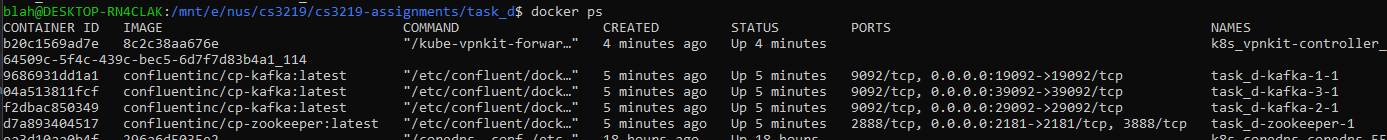
\includegraphics[width=\textwidth]{img/status.png}\\

    Create topic (\texttt{test-topic}):

    \texttt{docker exec -t task\_d-kafka-1-1 \textbf{kafka-topics --create --topic test-topic --zookeeper zookeeper:2181 --replication-factor 2 --partitions 3} }\\

    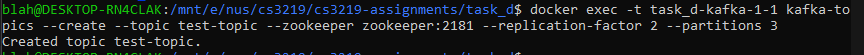
\includegraphics[width=\textwidth]{img/createTopic.png}\\

    Consume the message in node 2 (arbitrary):

    \texttt{docker exec -it task\_d-kafka-2-1 \textbf{kafka-console-consumer --bootstrap-server localhost:9092 --topic test-topic}}\\


    Send message in node 1 (aribitrary):

    \texttt{docker exec -it task\_d-kafka-1-1 \textbf{kafka-console-producer --broker-list localhost:9092 --topic test-topic}}

    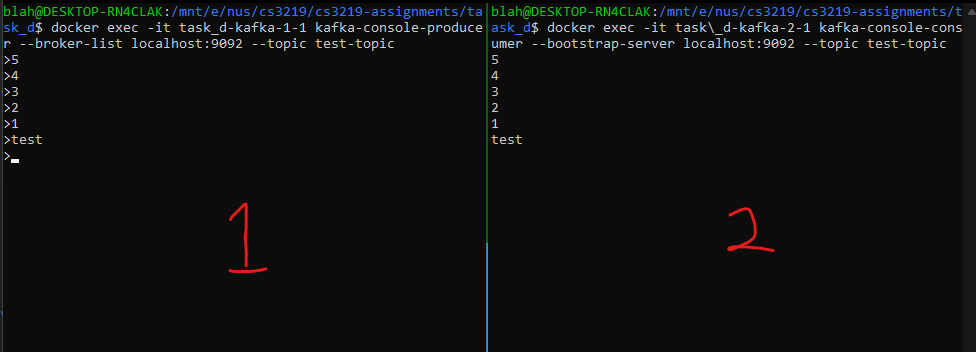
\includegraphics[width=\textwidth]{img/message.png}\\

    \pagebreak
    \section*{Failure management}

    View details of topics and their leaders:

    \texttt{docker exec -it task\_d-kafka-1-1 kafka-topics --zookeeper zookeeper:2181 --describe --topic test-topic}

    Kill one of the nodes:

    \texttt{docker kill task\_d-kafka-2-1}

    View details of topics and their leaders (again):

    \texttt{docker exec -it task\_d-kafka-1-1 kafka-topics --zookeeper zookeeper:2181 --describe --topic test-topic}

    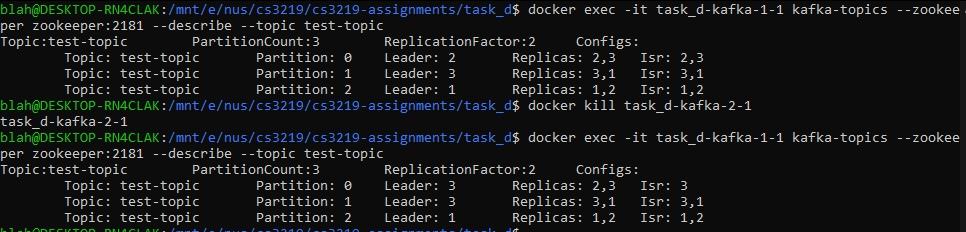
\includegraphics[width=\textwidth]{img/ded.png}\\

    Clearly, node 3 has taken over as leader of partition 0. To test this, once again,\\

    Consume the message in node 3:

    \texttt{docker exec -it task\_d-kafka-3-1 \textbf{kafka-console-consumer --bootstrap-server localhost:9092 --topic test-topic}}\\


    Send message in node 1:

    \texttt{docker exec -it task\_d-kafka-1-1 \textbf{kafka-console-producer --broker-list localhost:9092 --topic test-topic}}

    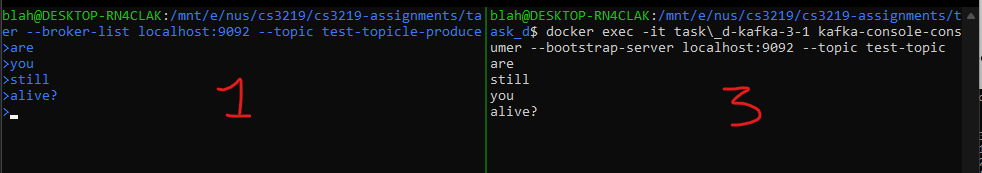
\includegraphics[width=\textwidth]{img/stillAlive.png}\\


    Interestingly, the latest \texttt{confluentinc/cp-kafka} image has finally deprecated \texttt{--zookeeper}, so I had to use an older image.

    \vspace*{\fill}
    Resources used:

    \href{https://medium.com/big-data-engineering/hello-kafka-world-the-complete-guide-to-kafka-with-docker-and-python-f788e2588cfc}{https://medium.com/big-data-engineering/hello-kafka-world-the-complete-guide-to-kafka-with-docker-and-python-f788e2588cfc}

    \href{https://www.baeldung.com/ops/kafka-docker-setup}{https://www.baeldung.com/ops/kafka-docker-setup}


\end{document}
